\documentclass[11pt]{article}


%%%%%%%%%%%%%%%%%%%%%%%%%%%%%%%%%%%%%%%%%%%%%%%%%%%%%%%%%%%%%%%%%%%%%%%%%%%%%%%%%%%%%%%%%%%%%%%%%%%%%%%%%%%%%%%%%%%%%%%%%%%%%%%%%%%%%%%%%%%%%%%%%%%%%%%%%%%%%%%%%%%%%%%%%%%%%%%%%%%%%%%%%%%%%%%%%%%%%%%%%%%%%%%%%%%%%%%%%%%%%%%%%%%%%%%%%%%%%%%%%%%%%%%%%%%%
\usepackage{amsfonts}
\usepackage{amsmath,amssymb,amsthm,enumerate,graphicx}
\usepackage{ifthen,latexsym,syntonly}
\usepackage{setspace}
\usepackage{mathabx}
\usepackage{color}
\usepackage[round,comma,authoryear]{natbib}
\usepackage{float}
\usepackage{epstopdf}
\usepackage{mathabx}
\usepackage{relsize}
\usepackage{color}
\usepackage{calc,xspace}
\usepackage{bibentry}
\usepackage{multirow}
\usepackage{graphicx}
\usepackage{xcolor}
\usepackage{subcaption}
\usepackage[stable]{footmisc} 
\setcounter{MaxMatrixCols}{10}
\usepackage{soul}
\usepackage{float}
\usepackage{booktabs}
\bibliographystyle{mynat}





\onehalfspacing

\bibpunct{(}{)}{,}{a}{}{,}  % for natbib
                            % need to have mynat.bst in an accesssible directory


\newtheorem{theorem}{Theorem}[section]
\newtheorem{remark}[theorem]{Remark}
\newtheorem{assumption}[theorem]{Assumption}
%\newtheorem{case}[theorem]{Case}
\newtheorem{claim}[theorem]{Claim}
%\newtheorem{conclusion}[theorem]{Conclusion}
\newtheorem{corollary}[theorem]{Corollary}
\newtheorem{condition}[theorem]{Condition}
\newtheorem{criterion}[theorem]{Criterion}
\newtheorem{definition}[theorem]{Definition}
\newtheorem{example}[theorem]{Example}
\newtheorem{lemma}[theorem]{Lemma}
\newtheorem{problem}[theorem]{Problem}
\newtheorem{proposition}[theorem]{Proposition}
%\newtheorem{solution}[theorem]{Solution}
%\newtheorem{summary}[theorem]{Summary}
\newtheorem{thm}[theorem]{Theorem}



\setlength{\oddsidemargin}{.05in} \setlength{\topmargin}{-.45in}
\setlength{\textwidth}{6.4in} \setlength{\textheight}{8.5in}

    
    \def\@fnsymbol#1{\ensuremath{\ifcase#1\or *\or \dagger\or \ddagger\or
    \mathsection\or \mathparagraph\or \|\or **\or \dagger\dagger
    \or \ddagger\ddagger \else\@ctrerr\fi}}

\renewcommand{\thefootnote}{\fnsymbol{footnote}}






\setcounter{page}{0}


\title{Updated plots}  

%\title{Wrestling with Uncertainty in \\ Climate Economic Models\footnotemark[3]}
%\vspace*{-0.3cm}
%{\fontsize{19}{30}\selectfont   
%Wrestling with Decision Theory }


%\author{Mike Barnett\footnote[3]\and William Brock\footnotemark[1] \and Lars Peter Hansen\footnotemark[7]}

%\footnotetext[3]{We thank Mike Barnett, Amy Boonstra, Diana Petrova and Bob Litterman for helpful comments on an earlier draft.} 

%\footnotetext[1]{University of Wisconsin and University of Missouri, Columbia}
%
%\footnotetext[7]{University of Chicago}
%
%\footnotetext[3]{Arizona State University}

\begin{document}

\maketitle
 
\section{Parameter setting: $\xi_w=1/600$, $\xi_a=1/10000$, $\xi_p=10\xi_w$, three damages ($1/3$, $1/3$, $1/3$ baseline probabilities)}

\subsection{Value function}
\begin{figure}[H]
		\center
		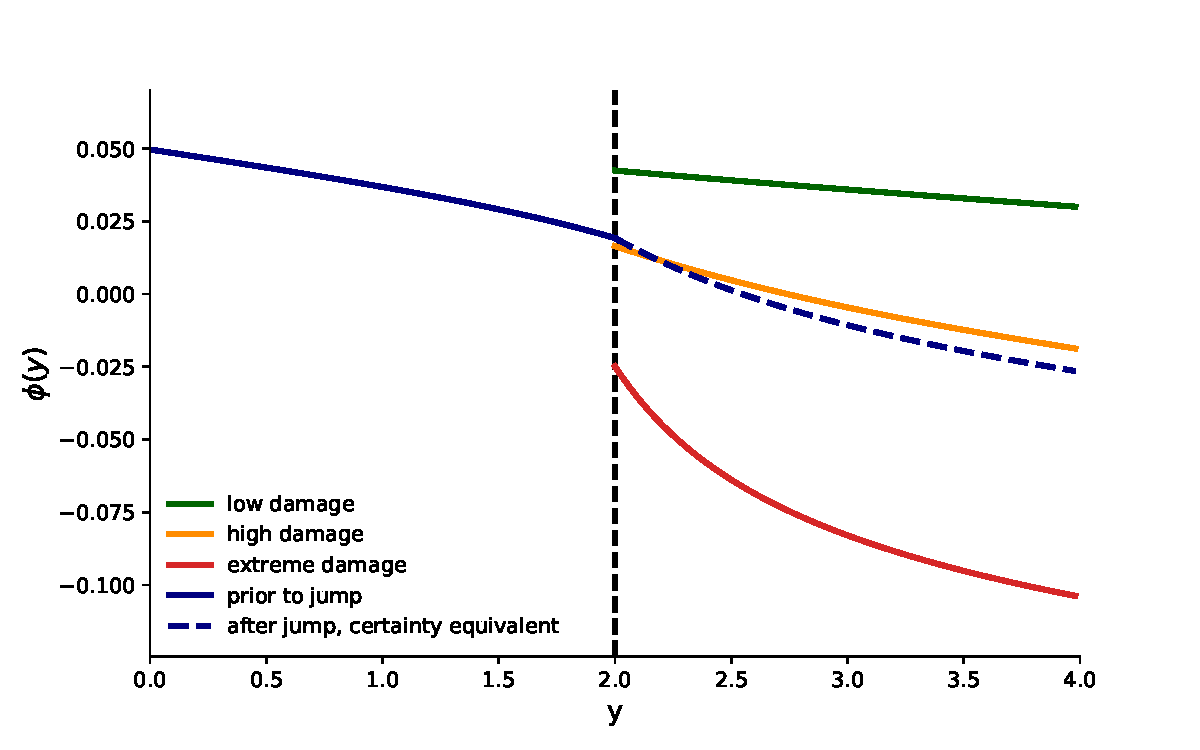
\includegraphics[height=.35\textheight]{value.pdf}
\end{figure}

\subsection{Emission and temperature change}
\begin{figure}[H]
		\center
		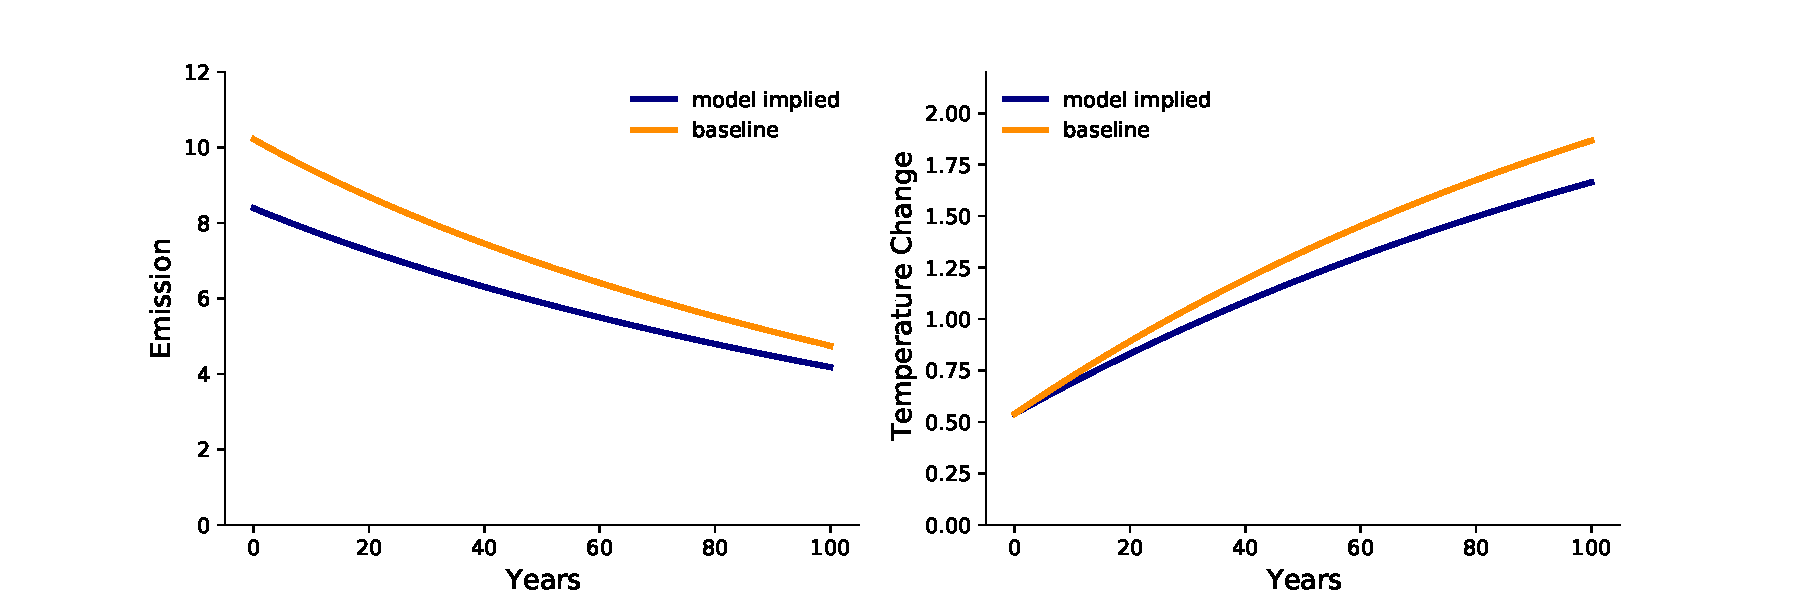
\includegraphics[height=.25\textheight]{emission_temperature.pdf}
\end{figure}

\subsection{Implied probabilities for damage function}
\begin{figure}[H]
		\center
		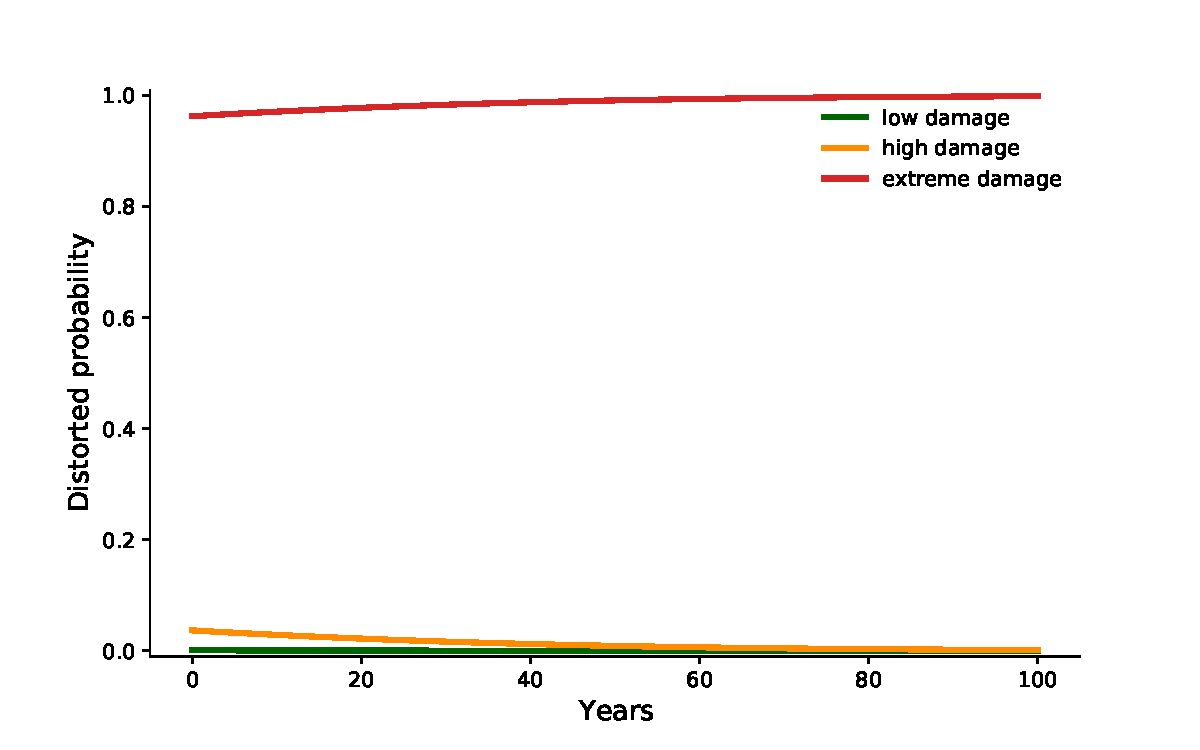
\includegraphics[height=.35\textheight]{damage_probability.pdf}
\end{figure}

\subsection{Histograms for climate sensitivities}
\begin{figure}[H]
		\center
		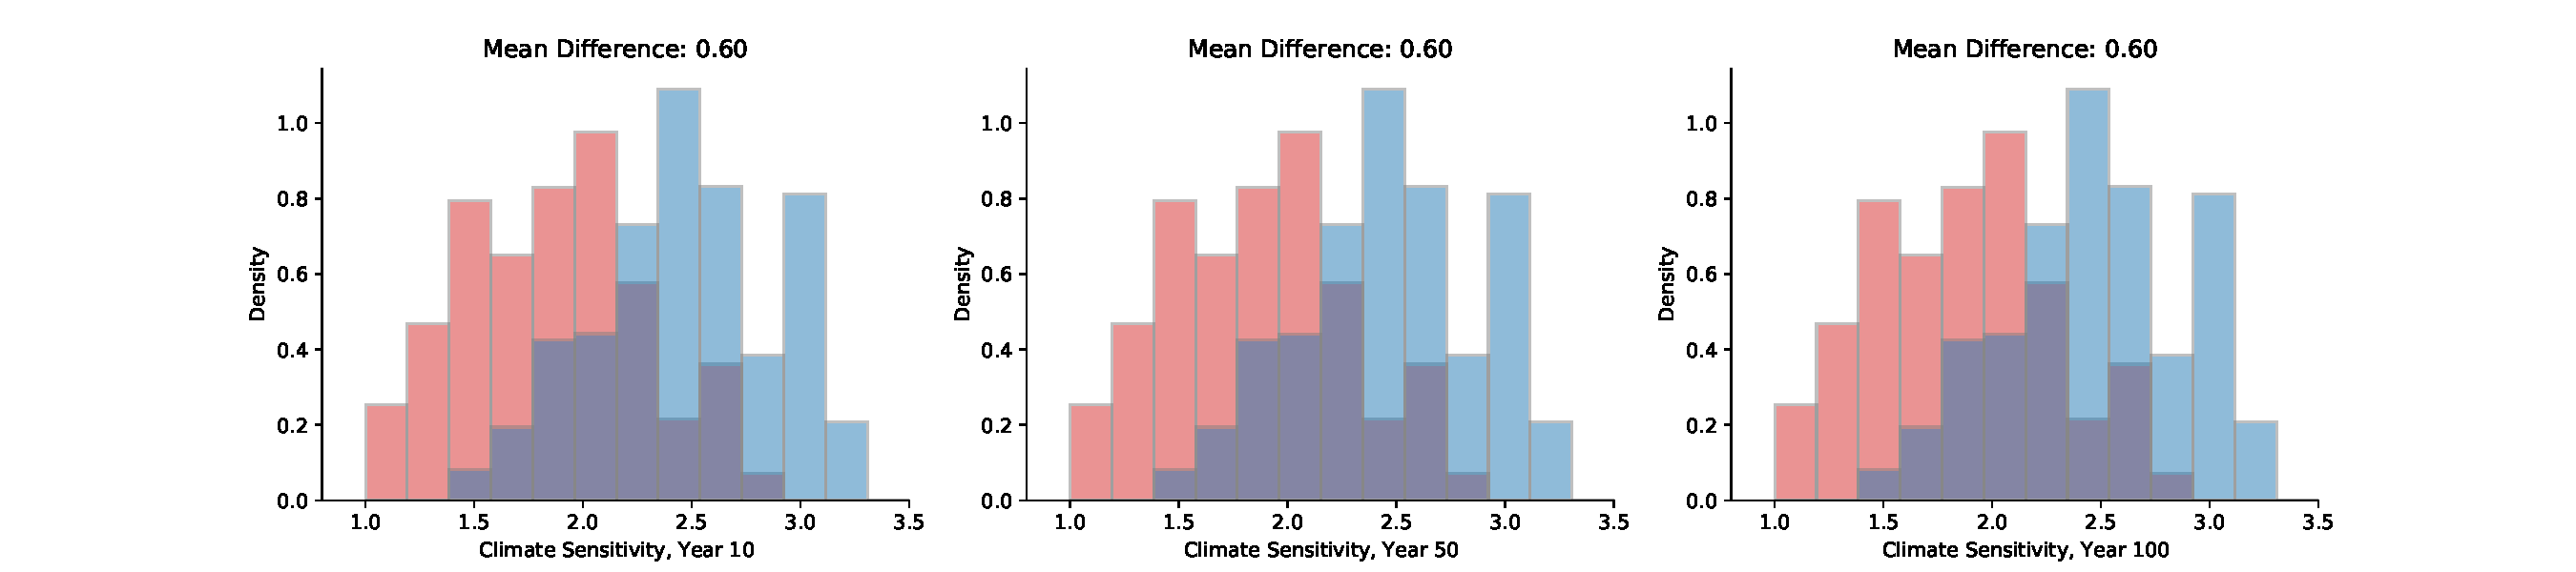
\includegraphics[height=.2\textheight]{climate_histogram.pdf}
\end{figure}

\subsubsection{Histograms for climate sensitivities (conditional on low damage)}

\begin{figure}[H]
		\center
		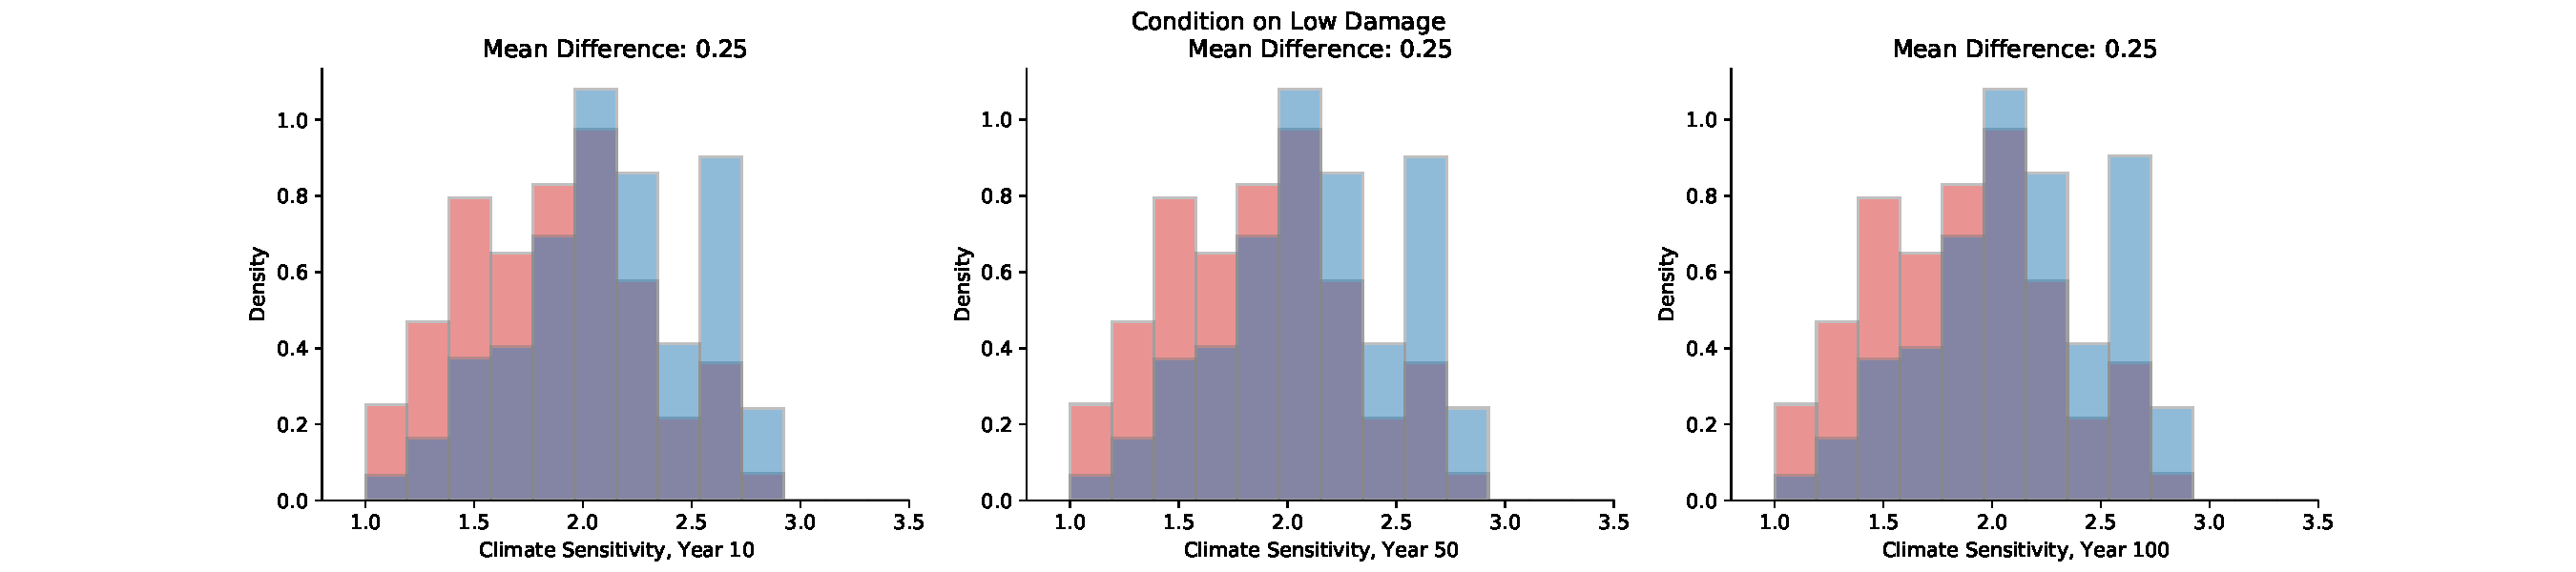
\includegraphics[height=.2\textheight]{climate_histogram_low_damage.pdf}
\end{figure}

\subsubsection{Histograms for climate sensitivities (conditional on high damage)}

\begin{figure}[H]
		\center
		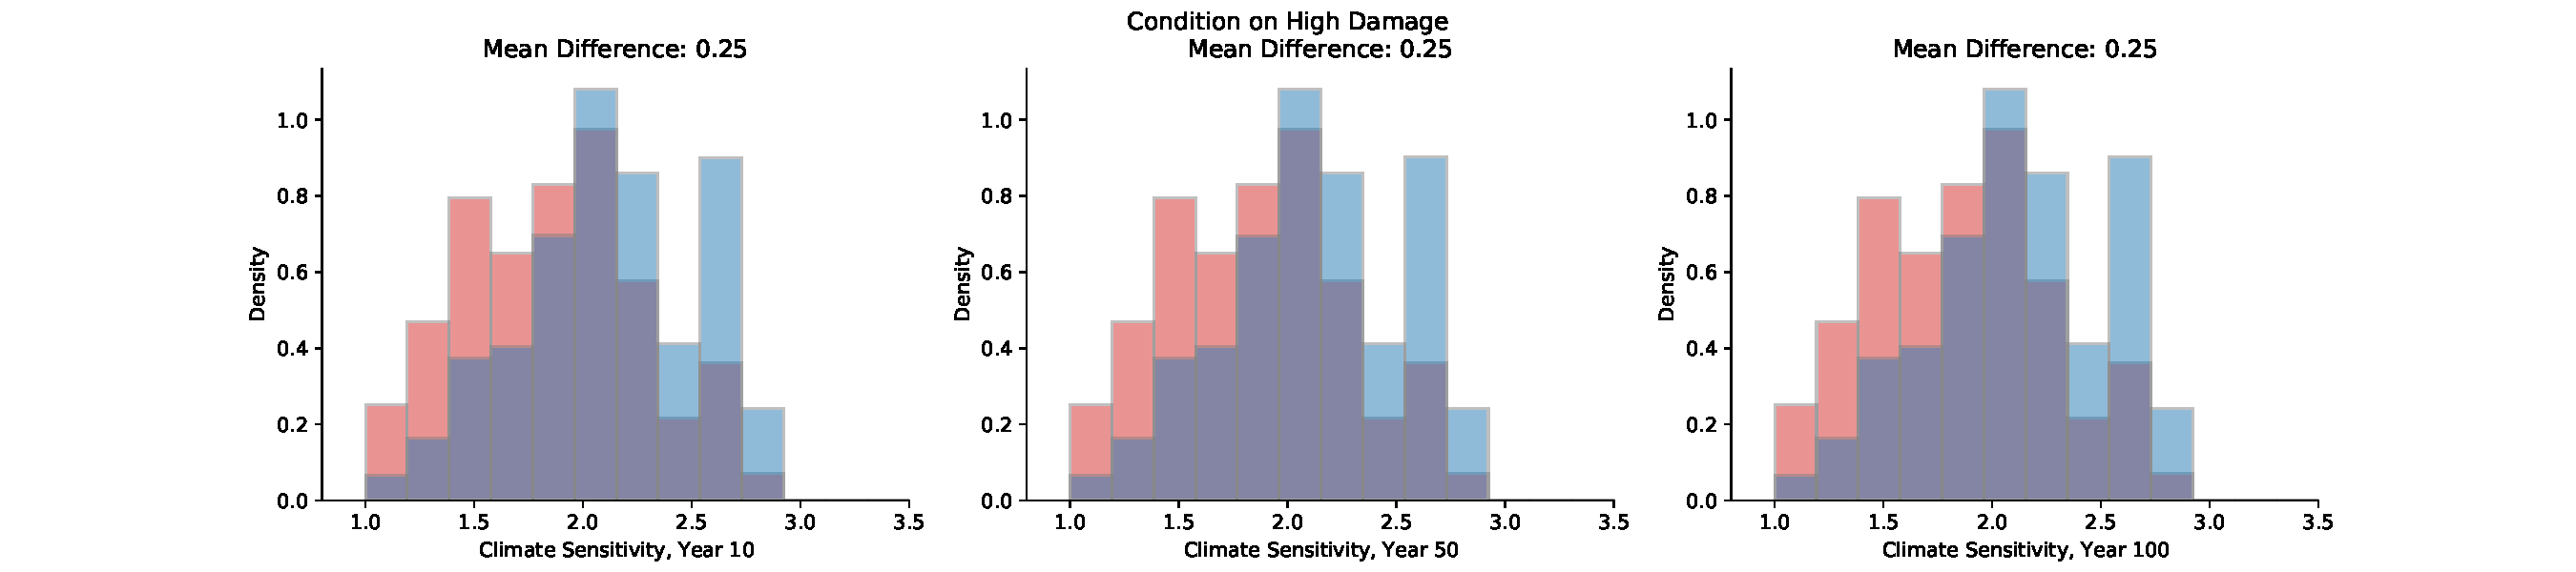
\includegraphics[height=.2\textheight]{climate_histogram_high_damage.pdf}
\end{figure}

\subsubsection{Histograms for climate sensitivities (conditional on extreme damage)}

\begin{figure}[H]
		\center
		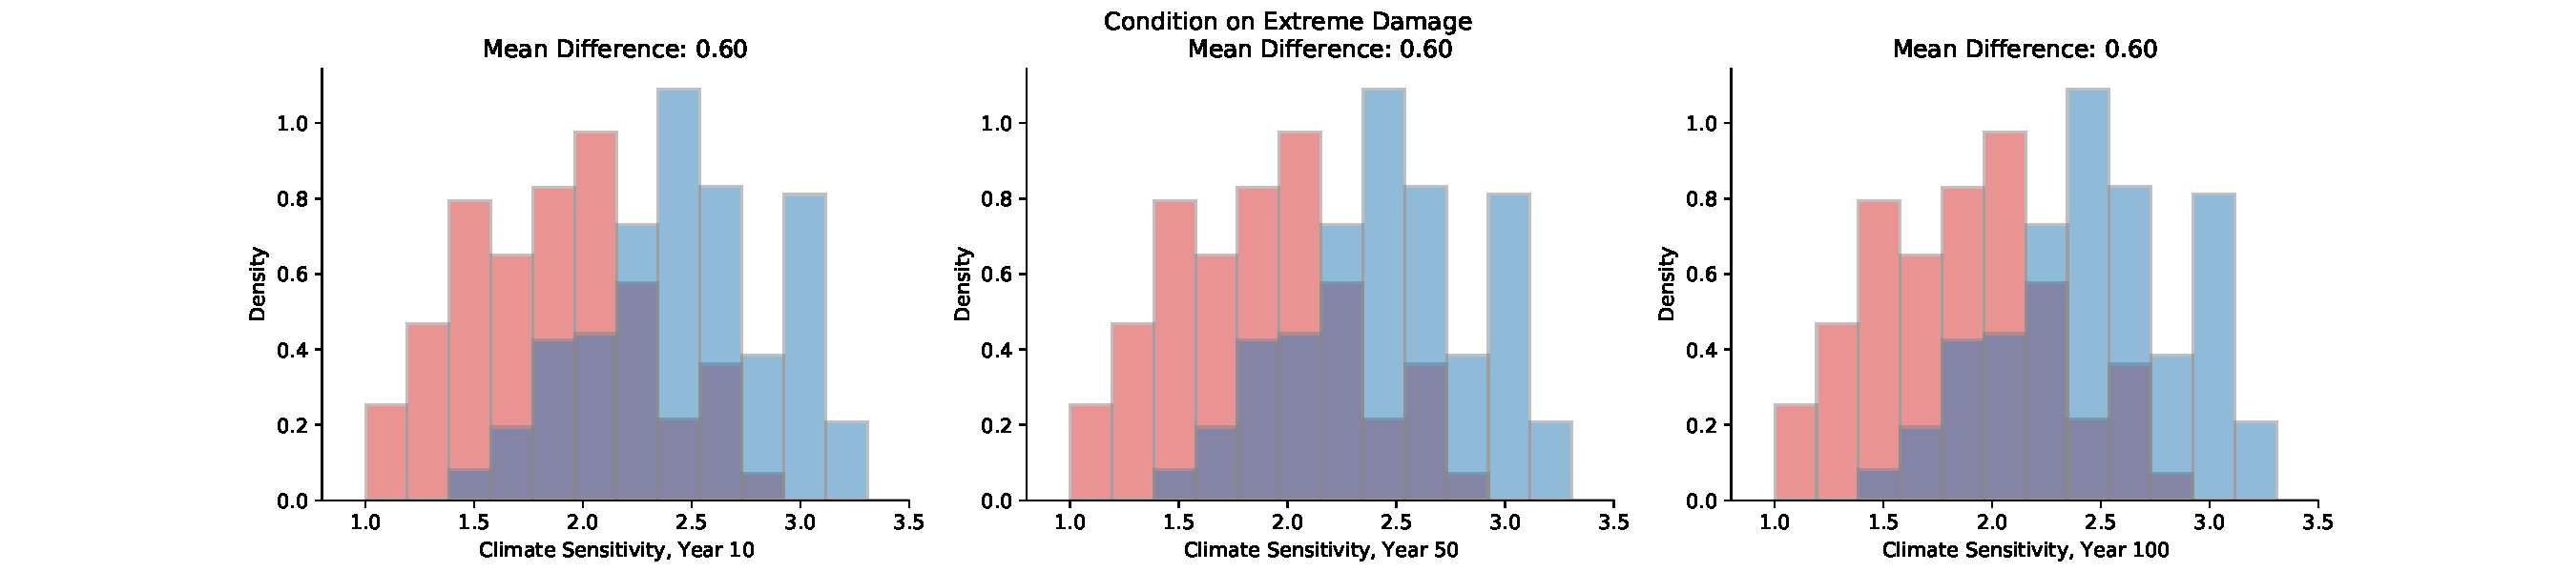
\includegraphics[height=.2\textheight]{climate_histogram_extreme_damage.pdf}
\end{figure}

\subsection{Marginal value of emission}
\begin{figure}[H]
		\center
		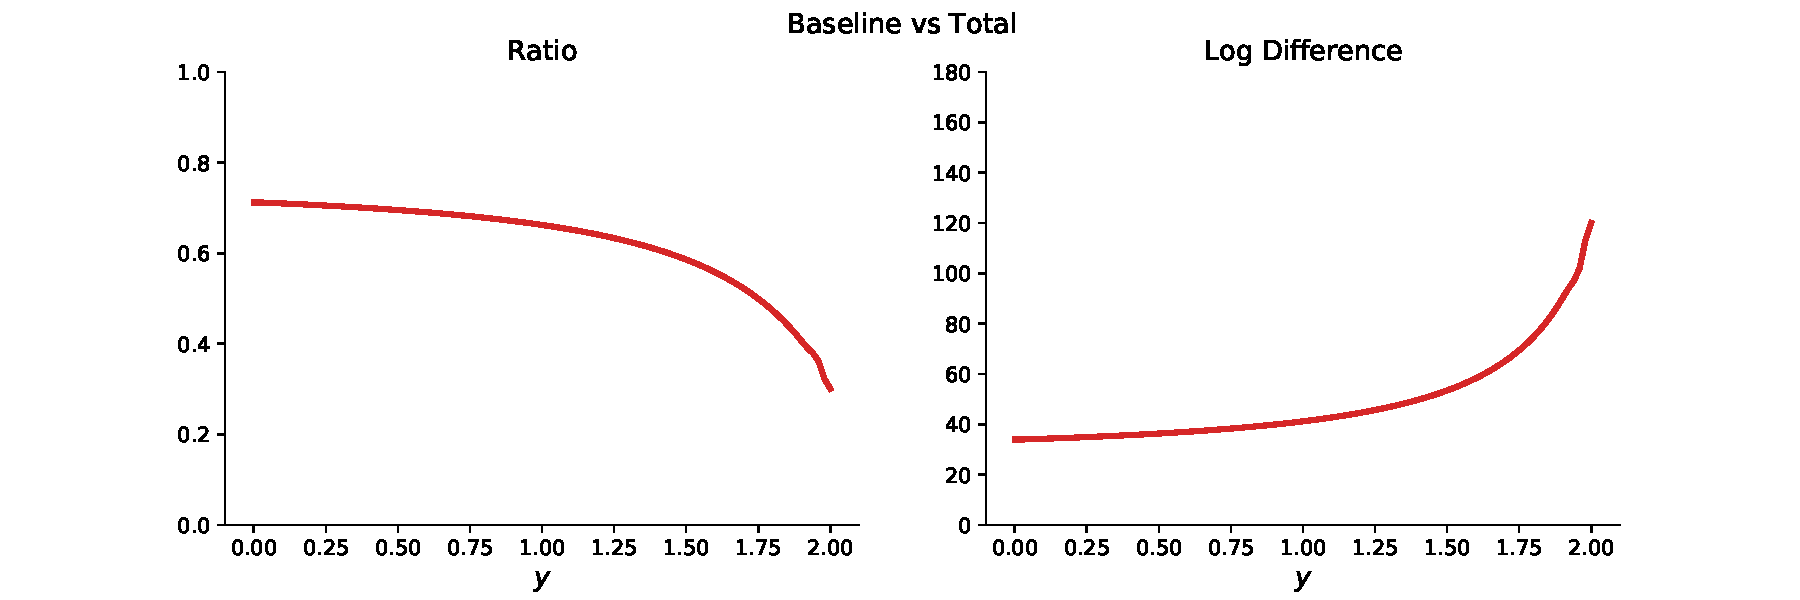
\includegraphics[height=.25\textheight]{me_baseline.pdf}
\end{figure}

\begin{figure}[H]
		\center
		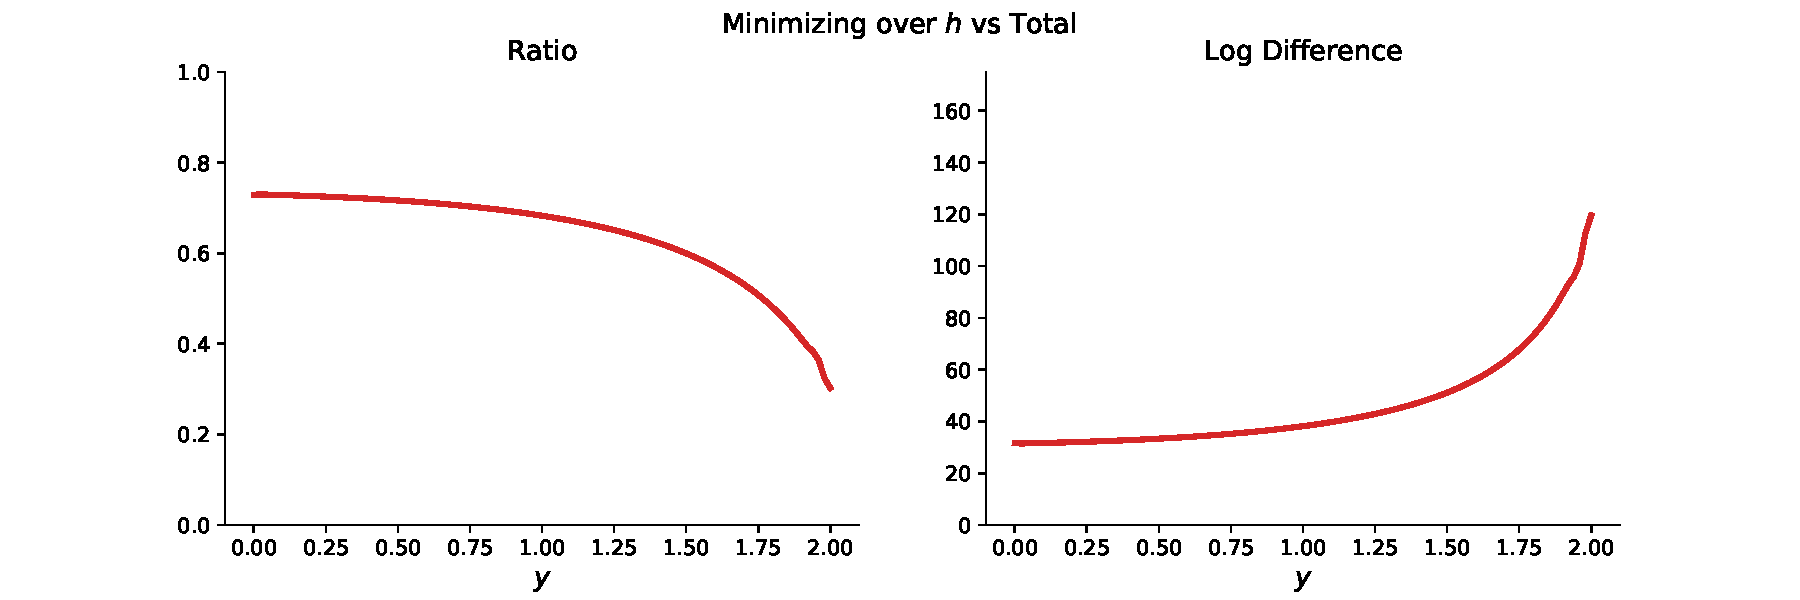
\includegraphics[height=.25\textheight]{me_min_w.pdf}
\end{figure}

\begin{figure}[H]
		\center
		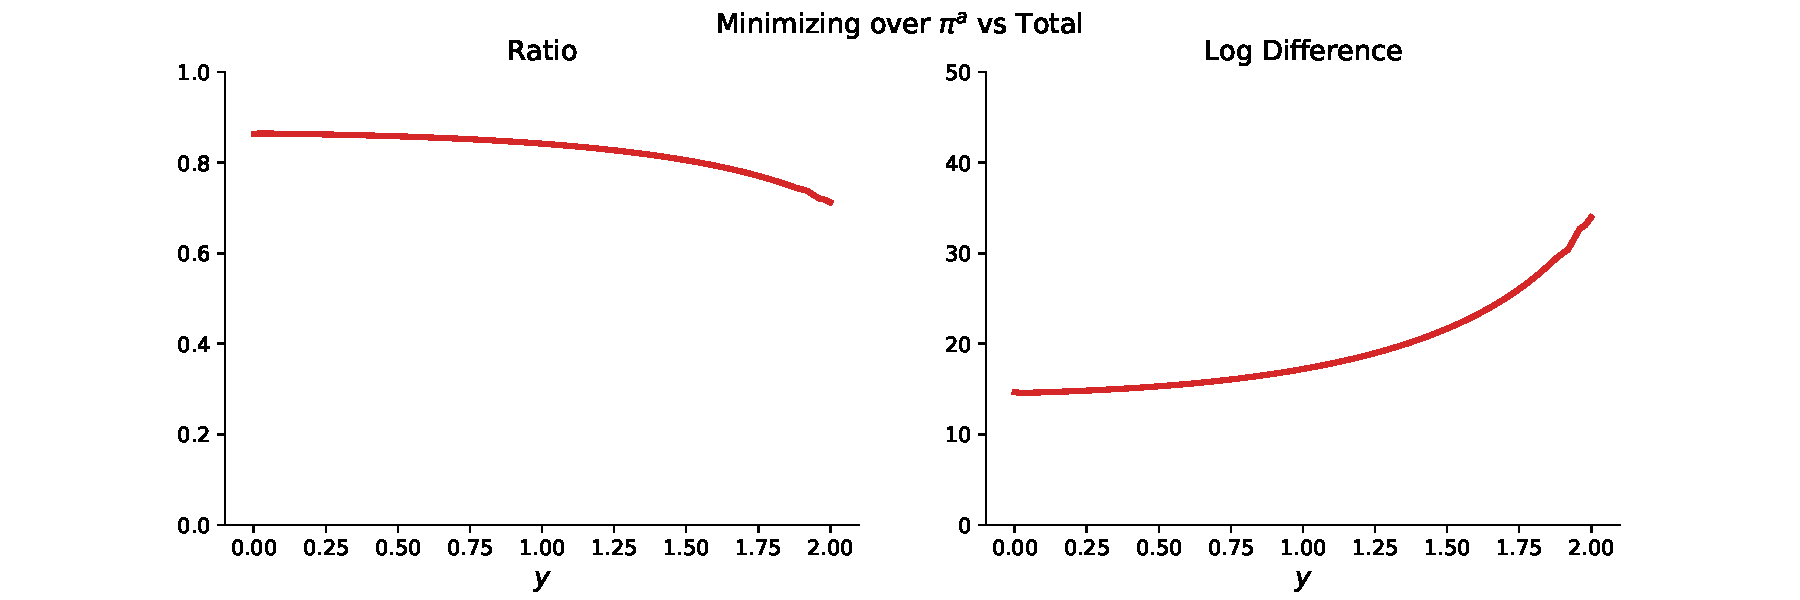
\includegraphics[height=.25\textheight]{me_min_a.pdf}
\end{figure}

\begin{figure}[H]
		\center
		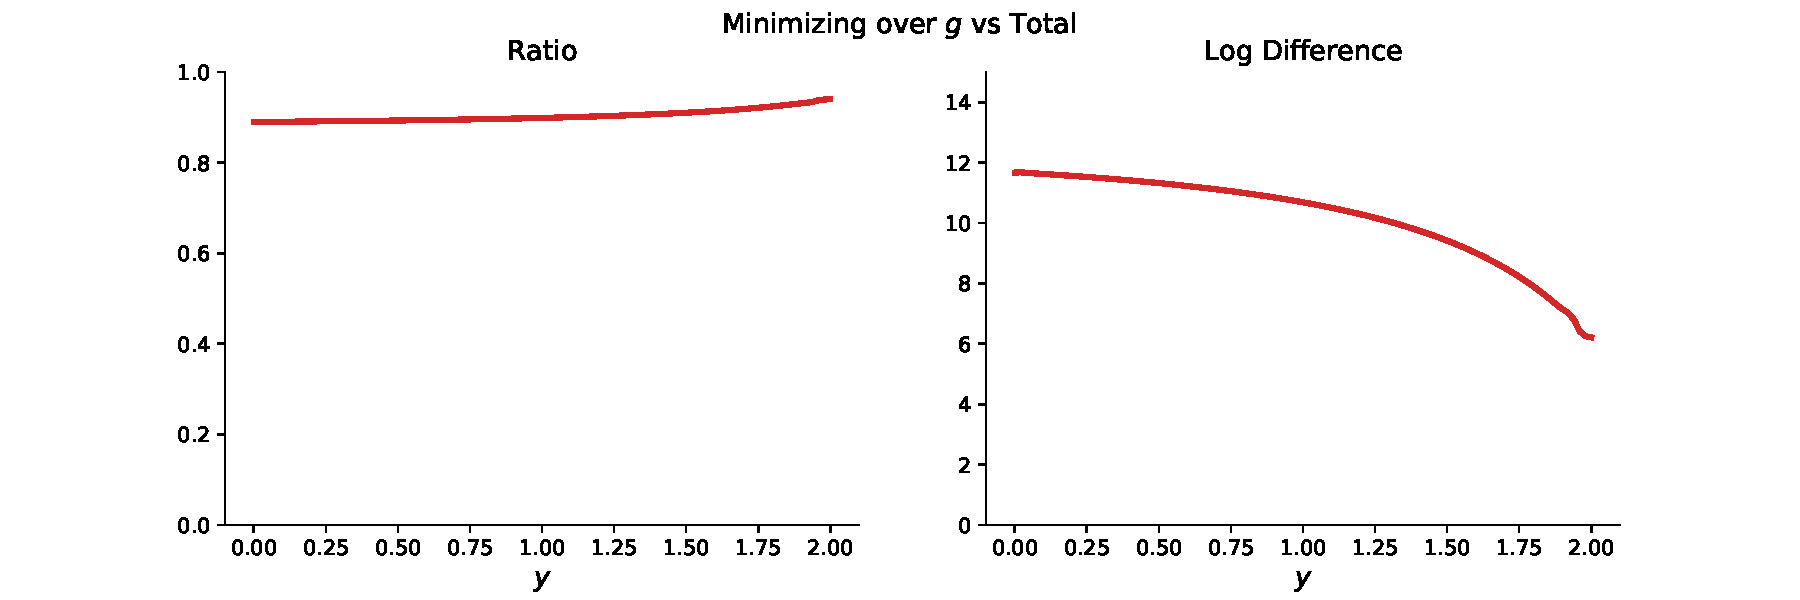
\includegraphics[height=.25\textheight]{me_min_p.pdf}
\end{figure}

\subsection{Social cost of carbon}
\begin{figure}[H]
		\center
		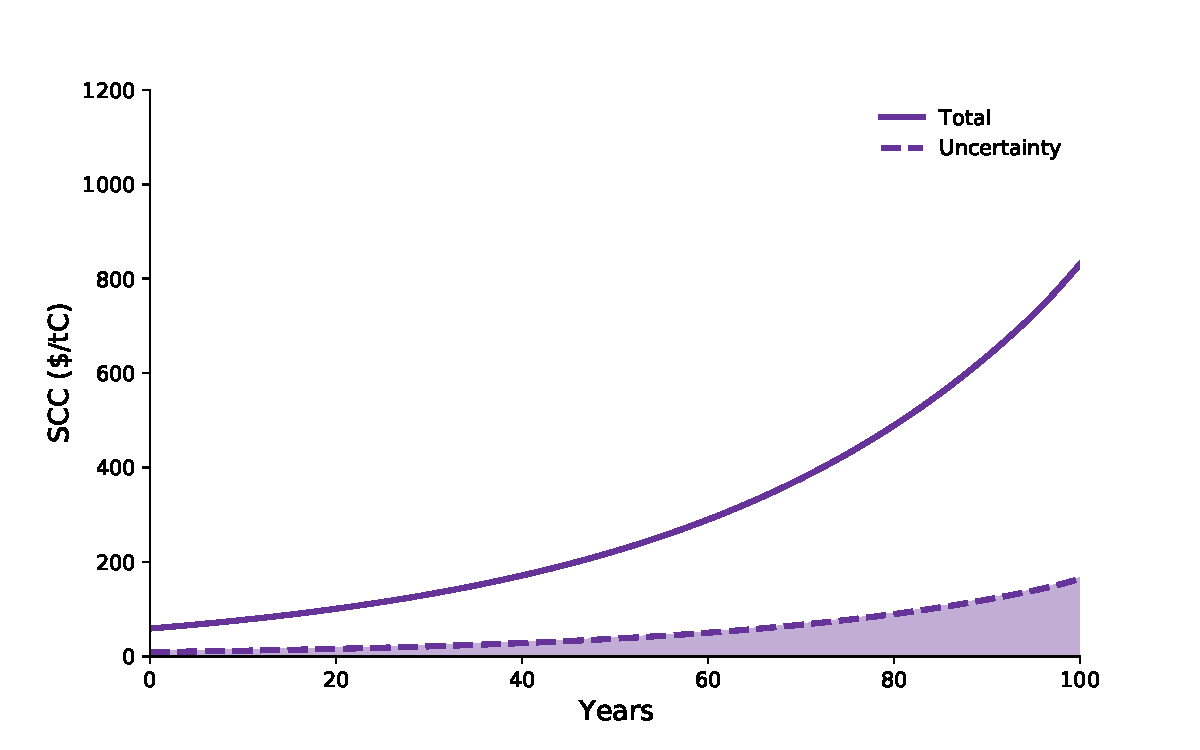
\includegraphics[height=.35\textheight]{scc.pdf}
\end{figure}

\end{document}



